\documentclass{article}
\usepackage{graphicx} % Required for inserting images
\usepackage[french]{babel}
\begin{document}
\title{Analyse de la méthode de fusion de boite WBF}
\date{Juin 2024}
\author{Hugo Dehurtevent}
\maketitle
\section{Comment fonctionne WBF}
Weighted Boxes Fusion (WBF) est une méthode de fusion de boite qui se base sur les scores de confidence de toutes les boites pour faire des boites moyennes. Le but est d'augmenter la qualité des boites.
\subsection{Comment cela fonctionne ?}
Supposons que nous avons un nombre N sorties de N modèles différents alors nous avons N prédictions de boites pour la même image.

Nous enregistrons chaque prédiction de boites dans une liste \textbf{B} qui est triés en fonction du score de confidence \textbf{C} de chaque boite par ordre décroissant.

Ensuite nous avons 2 autres liste, la liste \textbf{L} pour les cluster de boites, elle peut contenur une ou plusieurs boîtes par entrée. La Liste \textbf{F} qui nous permettra de stocker les résultats des fusions. 

Premièrement, nous devons faire un cycle dans notre liste \textbf{B}, on essaye de trouver un match dans la liste \textbf{F} en fonction du chevauchement avec la boîte en question (IoU > THR)(THR = optimal threshold).

S'il n'y a pas de match, on ajoute la boite de \textbf{B} à la fin de la liste \textbf{L} et \textbf{F}.

S'il y a un match alors, on ajoute notre boite à la liste \textbf{L} à la position correspondante de la liste \textbf{F}. Ensuite, nous devons recalculer le score de confiance, les valeurs de positions de notre boite de fusion et le remplacer dans \textbf{F} en utilisant toutes les boites accumulée à la même position dans la liste \textbf{L} en tant que \textbf{T}.

Pour ce faire nous pouvons le calculer comme ceci : 

\begin{itemize}
    \item Calcul du score de confidence: \(\frac{\sum_{i=1}^{T}C_i}{T}\)
    \item Calcul des x1,2: \(\frac{\sum_{i=1}^{T}C_i*x1,2_{i}}{\sum_{i=1}^{T}C_i}\)
    \item Calcul des y1,2: \(\frac{\sum_{i=1}^{T}C_i*y1,2_{i}}{\sum_{i=1}^{T}C_i}\)
\end{itemize}

Une fois toute la liste \textbf{B} parcourue, nous devons redimensionner les boites dans la liste \textbf{F}. Cela est nécessaire car le nombre de boite total dans le cluster à une certaine position peut être inférieur au nombre de modèle. Ce qui signifierais que peu de modèle l'on détecté. Pour faire le redimensionnement, nous avons deux méthode. 
\begin{enumerate}
    \item \(C = C * \frac{min(T,N)}{N}\)
    \item  \(C = C * \frac{T}{N}\)
\end{enumerate}

Il n'y a pas de différence majeur entre les deux méthodes seulement, il peut y avoir des clusters avec plus de boites que de modèles.

\section{Analyse des résultats}

Dans cette partie nous allons implémenter et analyser les résultats de la fusion avec la méthode WBF. 
Il y a plusieurs critères de mesure : 
\begin{itemize}
    \item La précision : représente le pourcentage de bonne détection par rapport à toute les détections.
    \item Le Recall : représente le pourcentage de bonne détection par rapport à la vérité terrain.
    \item le mAP : représente la moyenne des précision moyenne pour toutes les classes présentes dans le dataset. Il fournit une vue d'ensemble de la performance du modèle sur l'ensemble des classes.
\end{itemize}

\begin{table}[h!]
\centering
\begin{tabular}{|c||c|c|c|c||c|c|} 
\hline
Model & \multicolumn{3}{|c||}{BDD100K} & \multicolumn{3}{|c|}{COCO} \\ 
 & precision & recall & mAP  & precision & recall & mAP  \\ [0.5ex] 
\hline
Faster R-CNN & 0.6900 & 0.5331 & 14.2811 & 0.5881 & 0.7857 & 53.3767 \\ 
\hline
RetinaNet & 0.9028 & 0.3176 & 10.9700 & 0.8415 & 0.5504 & 54.7104 \\ 
\hline
FCOS & 0.8225 & 0.3962 & 12.5330 & 0.6908 & 0.6541 & 45.4001 \\ 
\hline
F R-CNN, RNet Cat & 0.6615 & 0.5348 & 10.8924 & 0.5479 & 0.7927 & 48.0539 \\ 
\hline
F R-CNN, RNet NMS & 0.6797 & 0.5336 & 10.5462 & 0.5840 & 0.7885 & 46.2454 \\ 
\hline
F R-CNN, RNet WBF & 0.6802 & 0.5336 & 8.5487 & 0.5845 & 0.7899 & 45.1434 \\ 
\hline
F R-CNN, FCOS Cat & 0.6270 & 0.5462 & 11.5580 & 0.4898 & 0.8095 & 47.4916 \\ 
\hline
F R-CNN, FCOS NMS & 0.6588 & 0.5405 & 10.9920 & 0.5564 & 0.8081 & 46.7206 \\ 
\hline
F R-CNN, FCOS WBF & 0.6616 & 0.5428 & 8.3086 & 0.5585 & 0.8095 & 45.3989 \\ 
\hline
RNet, FCOS Cat & 0.7742 & 0.4105 & 8.7381 & 0.6310 & 0.6779 & 41.1140 \\ 
\hline
RNet, FCOS NMS & 0.8100 & 0.4082 & 9.5651 & 0.6814 & 0.6709 & 42.1277 \\ 
\hline
RNet, FCOS WBF & 0.8079 & 0.4076 & 9.5906 & 0.6841 & 0.6765 & 44.4389 \\ 
\hline
F R-CNN, RNet, FCOS Cat & 0.6189 & 0.5462 & 9.0115 & 0.4614 & 0.8109 & 48.2450 \\ 
\hline
F R-CNN, RNet, FCOS NMS & 0.6522 & 0.5410 & 10.9920 & 0.5516 & 0.8081 & 46.7206 \\ 
\hline
F R-CNN, RNet, FCOS WBF & 0.6545 & 0.5410 & 7.8617 & 0.5543 & 0.8081 & 44.9204 \\ 
\hline
\end{tabular}
\caption{100 images avec filtre de 0.5 de confiance avant l'application du wbf}
\label{table:data}
\end{table}

Nous pouvons voir que lors de l'application du WBF, nous avons généralement une amélioration de précision par rapport à la fusion avec seulement de la concaténation et l'application du NMS. Le recall est généralement améliorer par rapport aux deux autres méthodes de fusion. Cependant nous avons un mAP qui est moins bon que sur les autres méthodes de fusions. 
\newpage
\subsection{Différence visible sur les méthodes de fusions}
Nous pouvons voir que dans certains cas, la méthode de fusion améliore ou non le score de précision, le recall et le mAP. 


Pour analyser son impacte, nous allons prendre des cas particulier et essayer de comprendre ce qui impacte ou non l'amélioration de nos résultats.


\begin{figure}[htp]
    \centering
    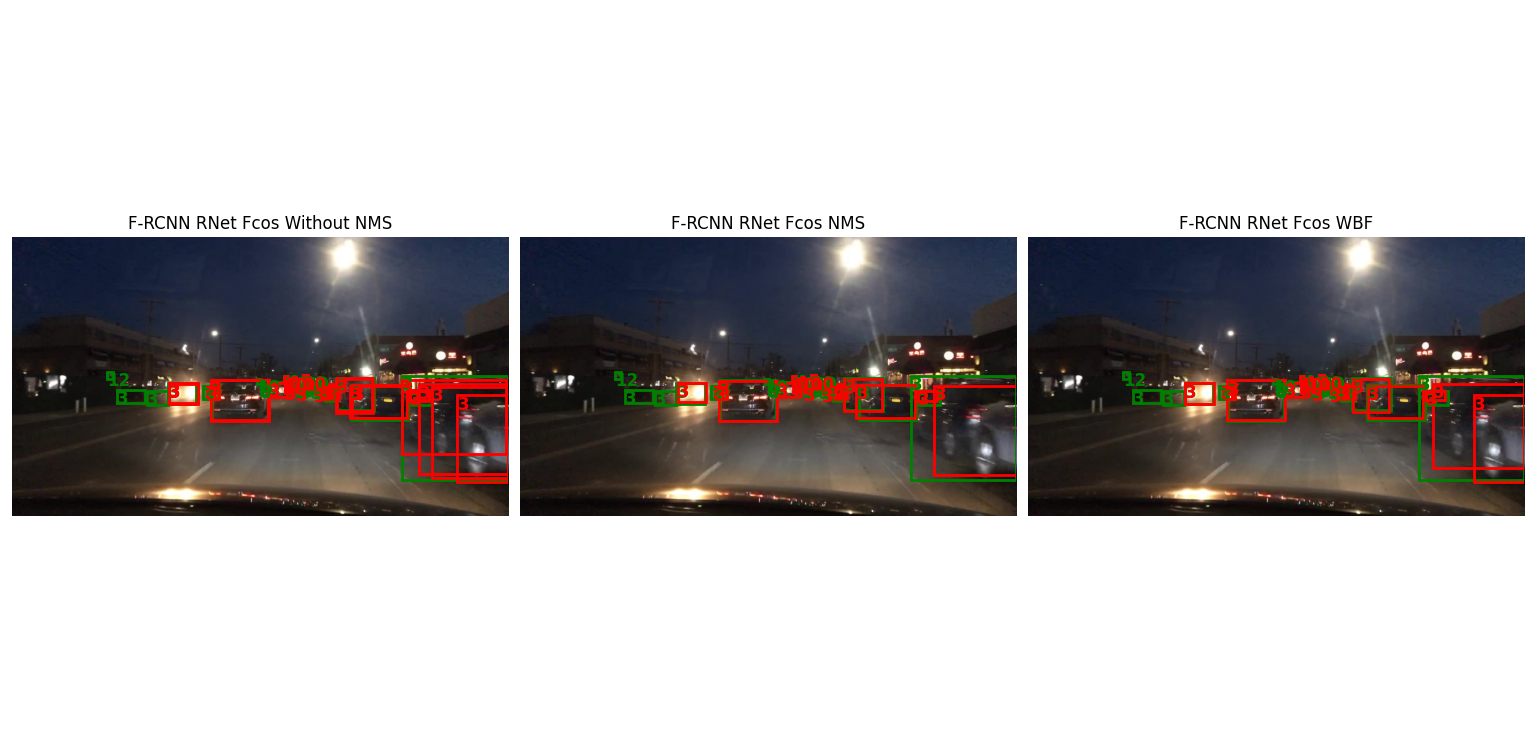
\includegraphics[width=1.3\textwidth]{images/Comparaison3FoixMemeImageFRCNNRNET.png}
    \caption{Image 24 de BDD100K}
    \label{fig:galaxy}
\end{figure}


Dans cette image, nous pouvons voir les rôles des différentes méthodes de fusions de modèles. Les résultats de précision, recall liée à cette images sont :

\begin{table}[h!]
    \centering
    \begin{tabular}{|c|c|c|c|c|c|}
        \hline
        \multicolumn{2}{|c|}{Cat} &\multicolumn{2}{|c|}{NMS} & \multicolumn{2}{|c|}{WBF} \\
        \hline 
         Precision & recall & Precision & recall & Precision & recall \\
         \hline 
         0.8148 & 0.6471 & 0.7500 & 0.5000 & 0.7059 & 0.5000 \\ 
    \hline
    \end{tabular}
    \caption{Scores for Image 24}
    \label{tab:my_label}
\end{table}

La première image correspond à la fusion avec concaténation des 3 sorties de nos modèles. La deuxième image correspond à la fusion avec l'application du NMS. Et la dernière correspond à la fusion avec l'application du WBF.
Nous pouvons voir que dans la première image, à droite nous avons plusieurs beaucoup de boite prédite pour les deux voitures. Selon la vérité terrain nous avons une seule détection. Dans ce cas la, nous pouvons voir que la fusion avec NMS remplis bien son rôle et laisse une seule détection. La fusion avec WBF sort 2 boites en fonction du score de confiance des boites. 

Nous pouvons voir que la fusion avec concaténation sort une précision et un recall meilleurs que les deux autres méthodes car il y a plus de boites prédite ce qui augmente le nombre de vrai prédiction tout en laissant un nombre faible de faux négatif. Les deux autres méthodes ont réduit considérablement le nombre de boites prédite, partant de 27 à 16 et 17 respectivement. La technique de fusion avec le NMS à réduit de un les faux positif comparé à la fusion avec WBF.

\begin{figure}[htp]
    \centering
    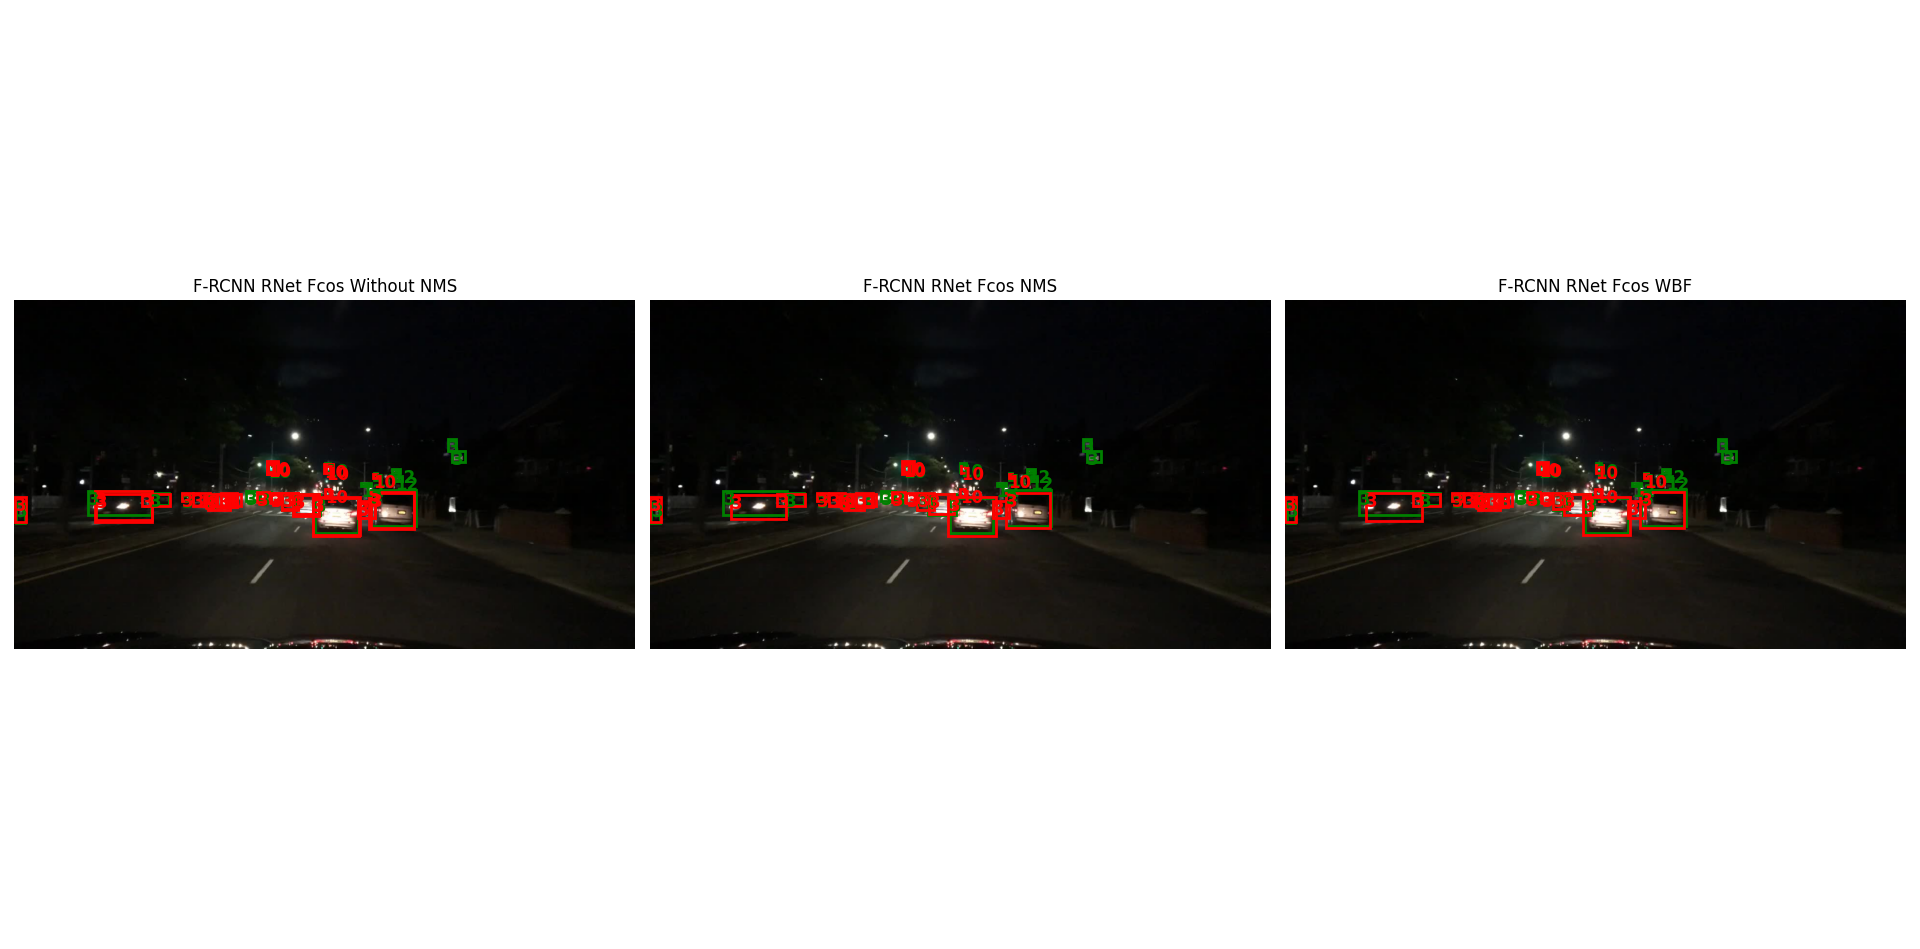
\includegraphics[width=1.3\textwidth]{images/Figure_8.png}
    \caption{Image 8 de BDD100K}
    \label{fig:galaxy}
\end{figure}

\begin{table}[h!]
    \centering
    \begin{tabular}{|c|c|c|c|c|c|}
        \hline
        \multicolumn{2}{|c|}{Cat} &\multicolumn{2}{|c|}{NMS} & \multicolumn{2}{|c|}{WBF} \\
        \hline 
         Precision & recall & Precision & recall & Precision & recall \\
         \hline 
         0.4815 & 0.6842 & 0.5455 & 0.6316 & 0.5909 & 0.6842 \\ 
    \hline
    \end{tabular}
    \caption{Scores for image 8}
    \label{tab:my_label}
\end{table}

Sur cette image, nous avons le cas où la fusion avec WBF est meilleur que les deux autres types de fusion.

\subsection{Analyse des résultats sur tout le dataset}

Dans cette partie, nous allons analyser les résultats pour tous le dataset et observer l'évolution du mAP. Nous voulons avoir une bonne mAP ainsi que un bon recall et précision. D'après la littérature, la méthode de fusion WBF permet d'augmenter le mAP général de nos modèles. 
\section{Problème de WBF}

Les problèmes de l'algorithme de fusion WBF que j'ai pu recensé sont les suivants :
\begin{enumerate}
    \item Problème de dégradation des scores
    \item Faible rapidité 
    \item Dépendance aux scores de confiance
\end{enumerate}

Pour le problème de dégradation des scores, cela est dû au fait que s'il y a trop de mauvais score à la base, cela nous diminue énormément les scores de confiances finaux.

La fusion WBF à aussi un problème de rapidité, il est reporté dans la littérature d'être 3 fois moins rapide que les autres techniques. Attention cela peut être beaucoup plus en fonction de la taille du dataset. 

La fusion WBF fonctionne avec le score de confiance de nos prédictions. Si ces scores sont biaisés ou faux, la fusion risque de diminuer les performances.


\subsection{Solution imaginée}
Pour régler le problème de dépendance aux scores de confiance et le problème de dégradation des scores, une solution a été imaginée. Elle utiliserait un seuil adaptatif pour enlever les boites trop faibles. 
Le seuil adaptatif doit se baser sur les statistiques de scores pour gérer dynamiquement le seuil en fonction de l'image d'entrée. Le problème d'avoir un seul seuil pour tout le modèle est que, si nous avons un seuil trop élevé alors nous allons augmenter le nombre de faux négatif. Cependant, un seuil trop bas diminuerait énormément la précision de notre modèle et donc augmenterais le nombre de faux positifs.
L'idée derrière le seuil adaptatif est que cela pourrait théoriquement filtrer les boites trop basses en fonction de leurs scores de confiances sur chaque image dans le but d'augmenter le mAP final de notre modèle.

Pour faire un seuil adaptatif, plusieurs techniques ont été pensées : 
\begin{enumerate}
    \item Filtrage basé sur la moyenne et l'écart-type
    \item Filtrage basé sur la médiane
    \item Filtrage basé sur les percentiles 
\end{enumerate}
De plus, une fois, le seuil adaptatif définit, nous l'utiliserons pour réduire le score de confiance des boites en dessous du seuil définit. 

L'utilisation de la moyenne et de l'écart-type permet de prendre en compte la distribution des scores. Plus les valeurs sont dispersées plus le seuil est strict.

L'utilisation de la médiane en tant que seuil est une méthode qui permet de faire un filtrage simple et efficace pour du filtrage rapide en temps réel. Il permet aussi de s'adapter à la distribution des données de chaque image.

L'utilisation des percentiles est une méthode qui permet de récupérer un pourcentage de boite détecté dans une image. Il est efficace et s'adapte bien à la distribution des données des images. 

Une fois, notre seuil définit, nous allons ajuster les scores au lieu de les supprimer. Cela nous permettra de garder toutes les boites, mais de réduire le mauvais impacte des mauvais scores pour la fusion wbf. 
\newpage

\section{Expérimentation}
Pour tester notre solution, une implémentation a été faite avec une valeur par défaut de percentile de 0.75, une valeur par défaut de facteur de réduction de 0.5. Voici les résultats : 

\begin{table}[h!]
    \centering
    \begin{tabular}{|c||c|c|c||c|c|c|} 
    \hline
    Model & \multicolumn{3}{|c||}{BDD100K} & \multicolumn{3}{|c|}{COCO} \\ 
     & precision & recall & mAP  & precision & recall & mAP  \\ [0.5ex] 
    \hline
    F R-CNN & 0.3597 & 0.7339 & \textbf{24.4800} & 0.2664 & 0.9335 & \textbf{55.4553} \\ 
    \hline
    RetinaNet & 0.1504 & 0.8462 & 21.2390 & 0.2036 & 0.9801 & 50.2337 \\ 
    \hline
    FCOS & 0.2880 & 0.7763 & 18.5343 & 0.3097 & 0.9575 & 46.7434 \\ 
    \hline
    F R-CNN, RetinaNet WBF & 0.1478 & 0.8742 & 24.3792 & 0.1881 & 0.9856 & 55.8966 \\ 
    \hline
    F R-CNN, RetinaNet Filtre Moyenne 1 & 0.1480 & 0.8745 & 24.3824 & 0.1882 & 0.9856 & 55.9224 \\ 
    \hline
    F R-CNN, RetinaNet Filtre Moyenne 2 & 0.1475 & 0.8742 & 24.4757 & 0.1883 & 0.9861 & 56.0299 \\ 
    \hline
    F R-CNN, RetinaNet Filtre Mediane & 0.1476 & 0.8744 & 24.0444 & 0.1888 & 0.9861 & 55.9077 \\ 
    \hline
    F R-CNN, RetinaNet Filtre Percentile & 0.1478 & 0.8752 & 23.6582 & 0.1883 & 0.9857 & 55.9754 \\ 
    \hline
    F R-CNN, FCOS WBF & 0.2601 & 0.8183 & 22.5496 & 0.2477 & 0.9693 & 51.5305 \\ 
    \hline
    F R-CNN, FCOS Filtre Moyenne 1 & 0.2600 & 0.8182 & 22.5641 & 0.2600 & 0.9693 & 51.5273 \\ 
    \hline
    F R-CNN, FCOS Filtre Moyenne 2 & 0.2600 & 0.8187 & 22.5479 & 0.2482 & 0.9693 & 51.4218 \\ 
    \hline
    F R-CNN, FCOS Filtre Mediane & 0.2592 & 0.8180 & 22.5024 & 0.2477 & 0.9692 & 51.6454 \\ 
    \hline
    F R-CNN, FCOS Filtre Percentile & 0.2595 & 0.8170 & 22.6299 & 0.2470 & 0.9690 & 51.7753 \\ 
    \hline
    RNet, FCOS WBF & 0.1457 & 0.8596 & 20.6941 & 0.1988 & 0.9827 & 43.8737 \\ 
    \hline
    RNet, FCOS Filtre Moyenne 1 & 0.1457 & 0.8596 & 20.6947 & 0.1988 & 0.9827 & 43.8497 \\ 
    \hline
    RNet, FCOS Filtre Moyenne 2 & 0.1458 & 0.8596 & 20.6353 & 0.1993 & 0.9831 & 44.0868 \\ 
    \hline
    RNet, FCOS Filtre Mediane & 0.1457 & 0.8607 & 20.8526 & 0.1978 & 0.9831 & 44.4836 \\ 
    \hline
    RNet, FCOS Filtre Percentile & 0.1456 & 0.8618 & 20.7913 & 0.1976 & 0.9831 & 45.3195 \\ 
    \hline
    F R-CNN, RNet, FCOS WBF & 0.1466 & 0.8883 & 23.6689 & 0.1886 & 0.9879 & 54.0298 \\ 
    \hline
    F R-CNN, RNet, FCOS Filtre M 1 & 0.1466 & 0.8883 & 23.6557 & 0.1887 & 0.9879 & 54.0314 \\ 
    \hline
    F R-CNN, RNet, FCOS Filtre M 2 & 0.1464 & 0.8880 & 23.6377 & 0.1889 & 0.9879 & 54.0513 \\ 
    \hline
    F R-CNN, RNet, FCOS Filtre Med & 0.1466 & 0.8891 & 23.5678 & 0.1879 & 0.9879 & 54.3335 \\ 
    \hline
    F R-CNN, RNet, FCOS Filtre Percentile & 0.1463 & 0.8892 & 23.5980 & 0.1884 & 0.9876 & 54.2620 \\ 
    \hline
    \end{tabular}
    \caption{Evaluation des perfomances avec le filtre stats}
    \label{table:data}
\end{table}


De ce que nous pouvons observer, la méthode avec le filtre percentile est souvent la plus efficace et constante pour améliorer notre mAP. Pour mieux observer l'impacte des hyperparamètres sur le filtre percentile, nous allons faire des expériences en faisant varier nos paramètres et observer leurs impactes sur les résultats.

\newpage

\subsection{Analyse du facteur de persentile}

\begin{figure}[htp]
    \centering
    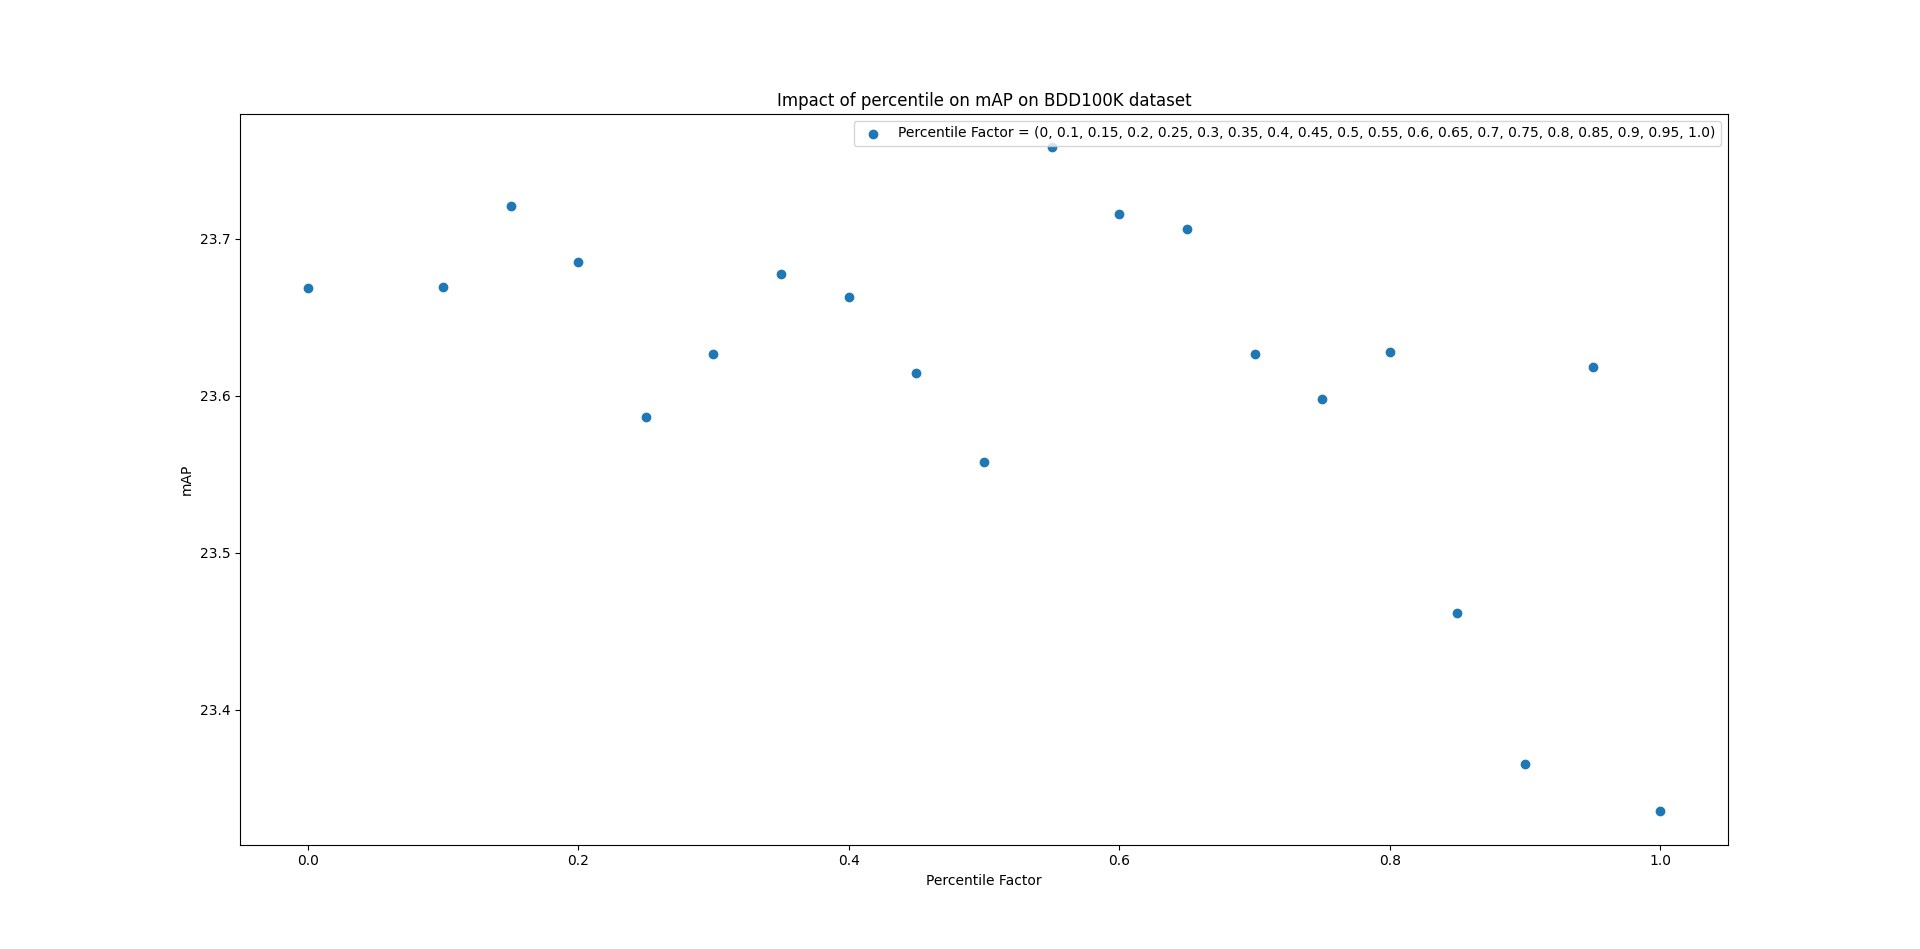
\includegraphics[width=1\textwidth]{images/Impacte des percentiles sur le dataset bdd100K.png}
    \caption{Variation du persentil pour BDD100K}
    \label{fig:galaxy}
\end{figure}

Pour le cas de BDD100K (Figure 3), nous pouvons voir que l'hyperparamètre percentile à beaucoup de fluctuation quand nous le faisons varier. Le point optimum de l'hyperparamètre est 0.55, c'est-à-dire que nous laissons 45 pourcents des meilleurs boites de chaque image intacte et que nous diminuons le score du reste des boites par 2. Les meilleures performances sont entre 0.0 et 0.4. Mais nous remarquons une légère tendance à la baisse quand nous dépassons 0.4.

\begin{figure}[htp]
    \centering
    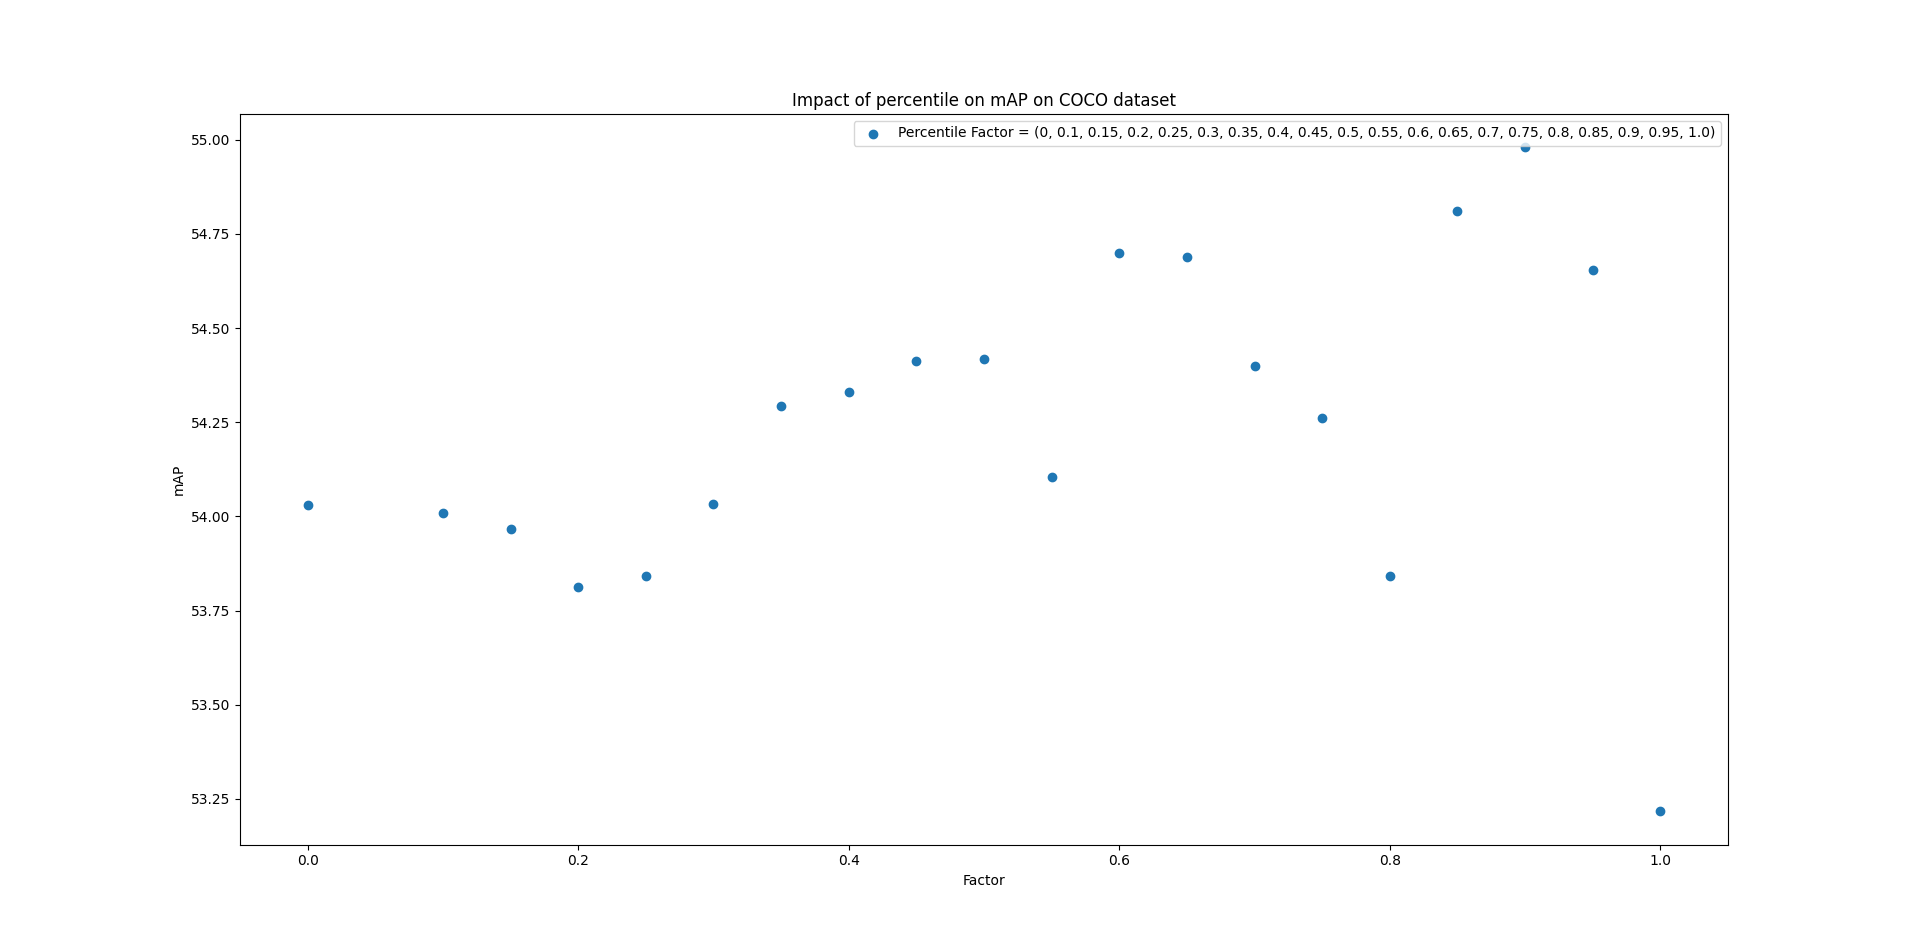
\includegraphics[width=1\textwidth]{images/Impacte des percentiles sur le dataset Coco.png}
    \caption{Variation du persentil pour COCO}
    \label{fig:galaxy}
\end{figure}

Pour le cas du dataset COCO (figure 4), notre mAP augmente de manière relativement linéaire avec l'augmentation du facteur jusqu'à 0.7. Les meilleures performances sont entre 0.6 et 0.7.


\subsection{Analyse du facteur de réduction}

\begin{figure}
    \centering
    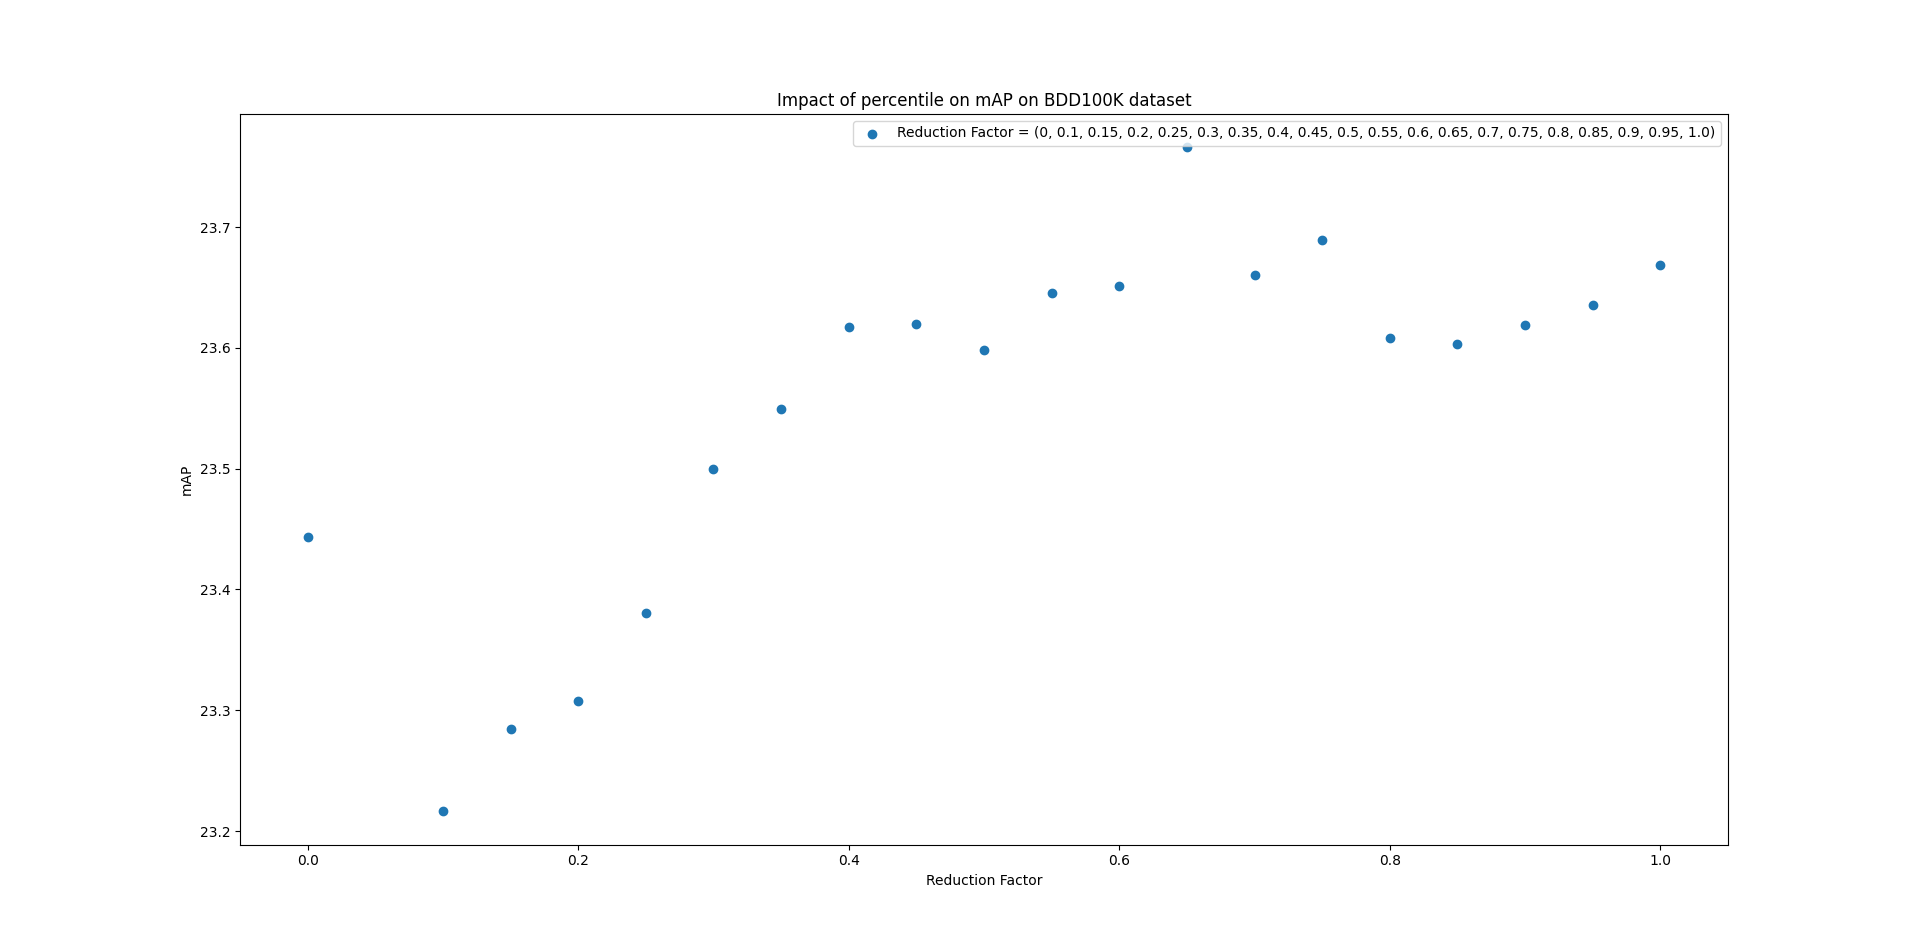
\includegraphics[width=1\textwidth]{images/Impacte du facteur de reduction sur le dataset bdd100K.png}
    \caption{Variation du facteur de réduction pour BDD100K}
    \label{fig:enter-label}
\end{figure}

Pour notre dataset BDD100K (figure 5), la map augmente de manière assez régulière avec l'augmentation du facteur de réduction, jusqu'à environ 0.5 - 0.6 puis commence à diminuer. Cela diminue notablement après 0.7.


\begin{figure}
    \centering
    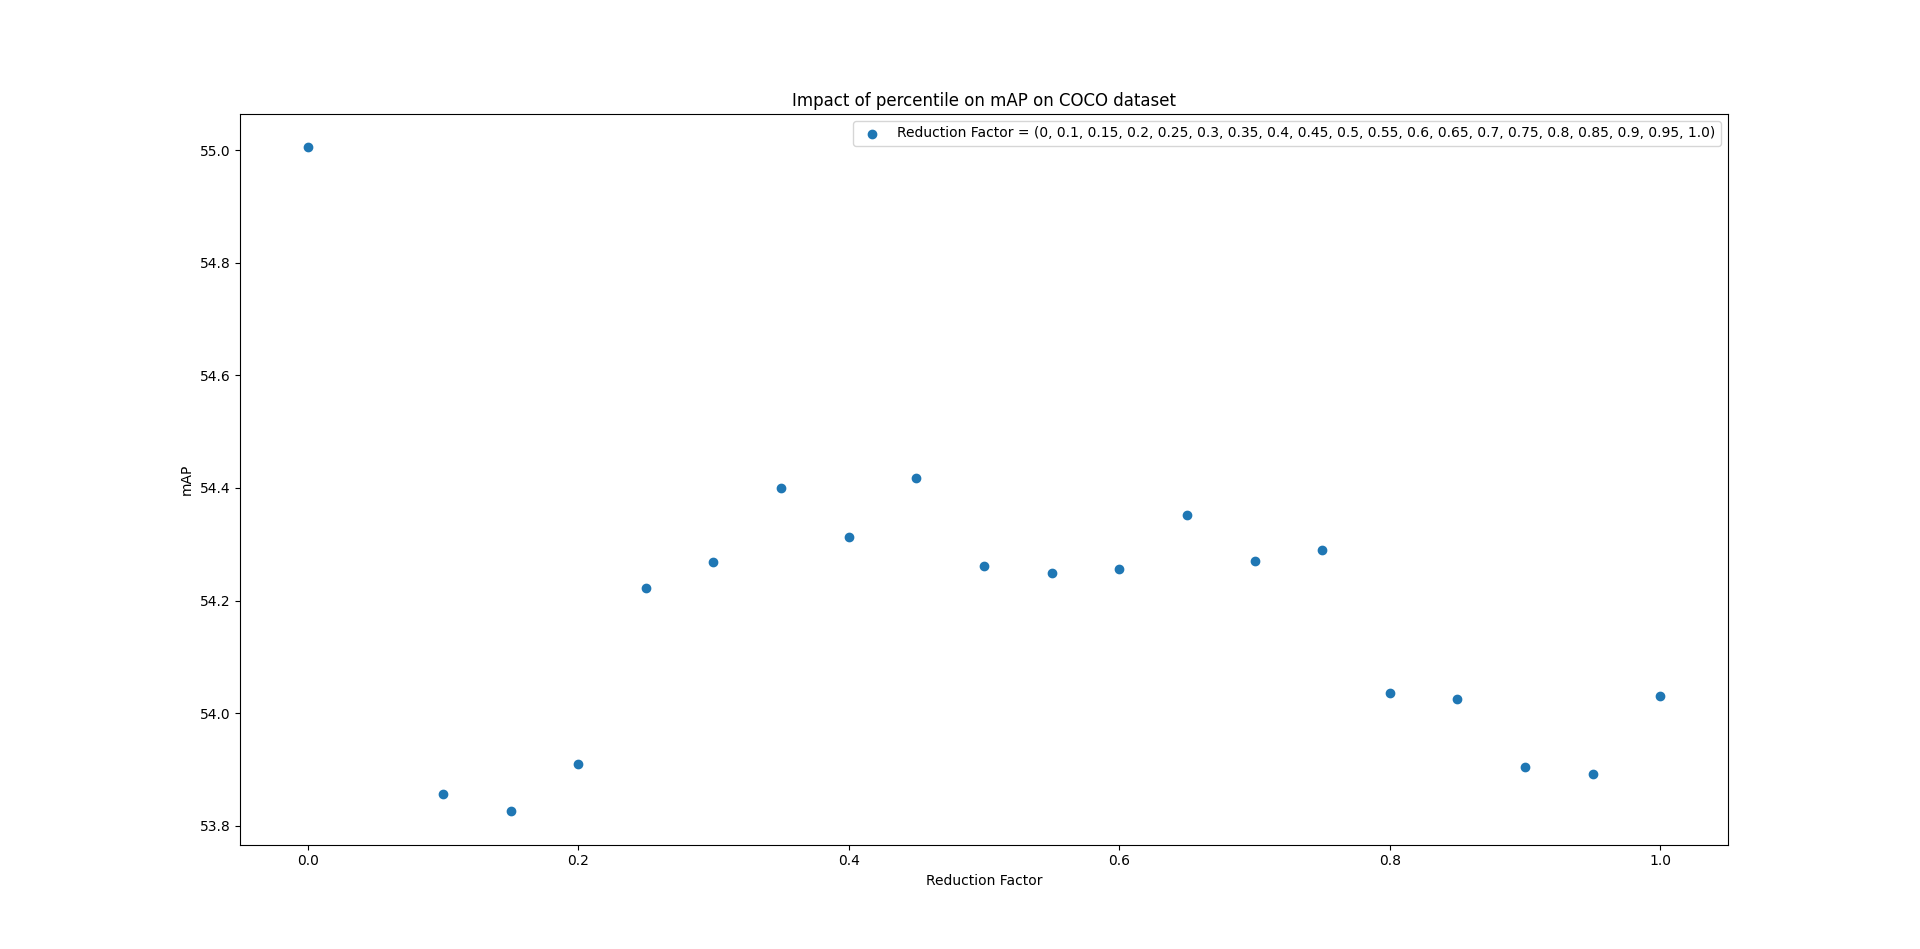
\includegraphics[width=1\textwidth]{images/Impacte du facteur de reduction sur le dataset Coco.png}
    \caption{Variation du facteur de réduction pour COCO}
    \label{fig:enter-label}
\end{figure}

Pour le dataset COCO (figure 6), la tendance est similaire à celle de BDD100K, avec une augmentation jusqu'à 0.5-0.6. Il y a une diminution prononcée à 1.0.


\newpage
\subsection{Observations générales}

Pour les deux datasets (BDD100K et COCO), les meilleurs résultats en termes de mAP sont obtenus avec des valeurs de facteurs de percentile et de réduction situées autour de 0.5-0.6.

Pour les deux datasets, les valeurs extrêmes (très basses ou très élevées) des percentiles et facteurs de réduction entraînent une diminution notable de la mAP.

Cette tendance indique qu'il y a probablement une limite à l'utilité de l'élimination ou de la pondération excessive des prédictions des modèles.
Les deux datasets réagissent différemment aux modifications des percentiles et des facteurs de réduction.
Le dataset COCO semble plus sensible aux modifications du percentile, avec une augmentation plus régulière de la mAP jusqu'à un certain point avant de diminuer, tandis que le dataset BDD100K montre une fluctuation plus imprévisible.


\subsection{Evaluation avec un filtre à 0.5}

\begin{table}[h!]
\centering
\begin{tabular}{|c||c|c|c||c|c|c|} 
\hline
Model & \multicolumn{3}{|c||}{BDD100K} & \multicolumn{3}{|c|}{COCO} \\ 
 & precision & recall & mAP  & precision & recall & mAP  \\ [0.5ex] 
\hline
F R-CNN & 0.6982 & 0.5432 & \textbf{22.8207} & 0.5934 & 0.7907 & \textbf{52.8998} \\ 
\hline
RetinaNet & 0.9026 & 0.3172 & 17.2830 & 0.8482 & 0.5469 & 39.8350 \\ 
\hline
FCOS & 0.8307 & 0.4100 & 16.1693 & 0.7179 & 0.6535 & 41.2791 \\ 
\hline
F R-CNN, RNet WBF & 0.8483 & 0.4138 & \textbf{20.6369} & 0.7545 & 0.6460 & \textbf{49.7903} \\ 
\hline
F R-CNN, RNet Filtre Percentile & 0.8841 & 0.3759 & 19.8248 & 0.7992 & 0.6017 & 48.2059 \\ 
\hline
F R-CNN, FCOS WBF & 0.8388 & 0.4580 & \textbf{20.0853} & 0.7170 & 0.6921 & \textbf{45.2107} \\ 
\hline
F R-CNN, FCOS Filtre Percentile & 0.8778 & 0.3844 & 18.2468 & 0.7738 & 0.5823 & 40.5647 \\ 
\hline
RNet, FCOS WBF & 0.9546 & 0.2631 & \textbf{14.9456} & 0.8711 & 0.4294 & \textbf{31.6934} \\ 
\hline
RNet, FCOS Filtre Percentile & 0.9468 & 0.2530 & 14.7225 & 0.8731 & 0.3989 & 30.2301 \\ 
\hline
F R-CNN, RetRNetinaNet, FCOS WBF & 0.9081 & 0.3825 & \textbf{19.7971} & 0.8049 & 0.5977 & \textbf{45.6442} \\ 
\hline
F R-CNN, RNet, FCOS Filtre Percentile & 0.9227 & 0.3343 & 18.7332 & 0.8623 & 0.5403 & 43.4242 \\ 
\hline
\end{tabular}
\caption{Evaluation des perfomances avec le filtre à 0.5 }
\label{table:data}
\end{table}

\end{document}